\section{Results and discussion}\label{sec:results}
The following chapter will discuss the results of the models presented in section~\ref{sec:methodology} before comparing the different models and discussing the results. We will start by examining the different ARIMA models, from the simplest ARIMA to the more complex SARIMAX. We will then compare this to the LSTM model. 

\subsection{ARIMA}\label{sec:arima}
As explained in section~\ref{ARIMA and SARIMAX Methodology}, determining the order of the ARIMA model can be a difficult and complex task, examining the ACF and PACF plots can be a good starting point, but will also be a bit subjective. The only objective way to optimize the model is to use a loss function. In our case we have chosen root mean squared error as this is a commonly used way to measure the accuracy of a model.

In order to find the model with the least RMSE, we performed a grid search on the different parameters using a nested for-loop and outputting the results in the following table: 
\begin{table}[H]
    \begin{center}
        \import{data/Figures/ARIMA/}{AutoARIMAResults}
        \caption{Results of the grid search for the ARIMA model.}\label{tab:ARIMAResults}
    \end{center}
\end{table}
Examining table~\ref{tab:ARIMAResults} we can see that the ARIMA(0,1,1) has the lowest RMSE and is therefore expected to be the best model, but there is no significant difference between the models. This may indicate that the model is not able to capture the trends. An ARIMA model with $p$ of 0, $d$ of 1 and $q$ of 1 is, according to \textcite{nau_2019}, a simple exponential smoothing model which indicates that it may capture the moving average trend, but no other trends. Fitting the model to the data and plotting the results against the actual values we get the following plot:
\begin{figure}[H]
    \begin{center}
        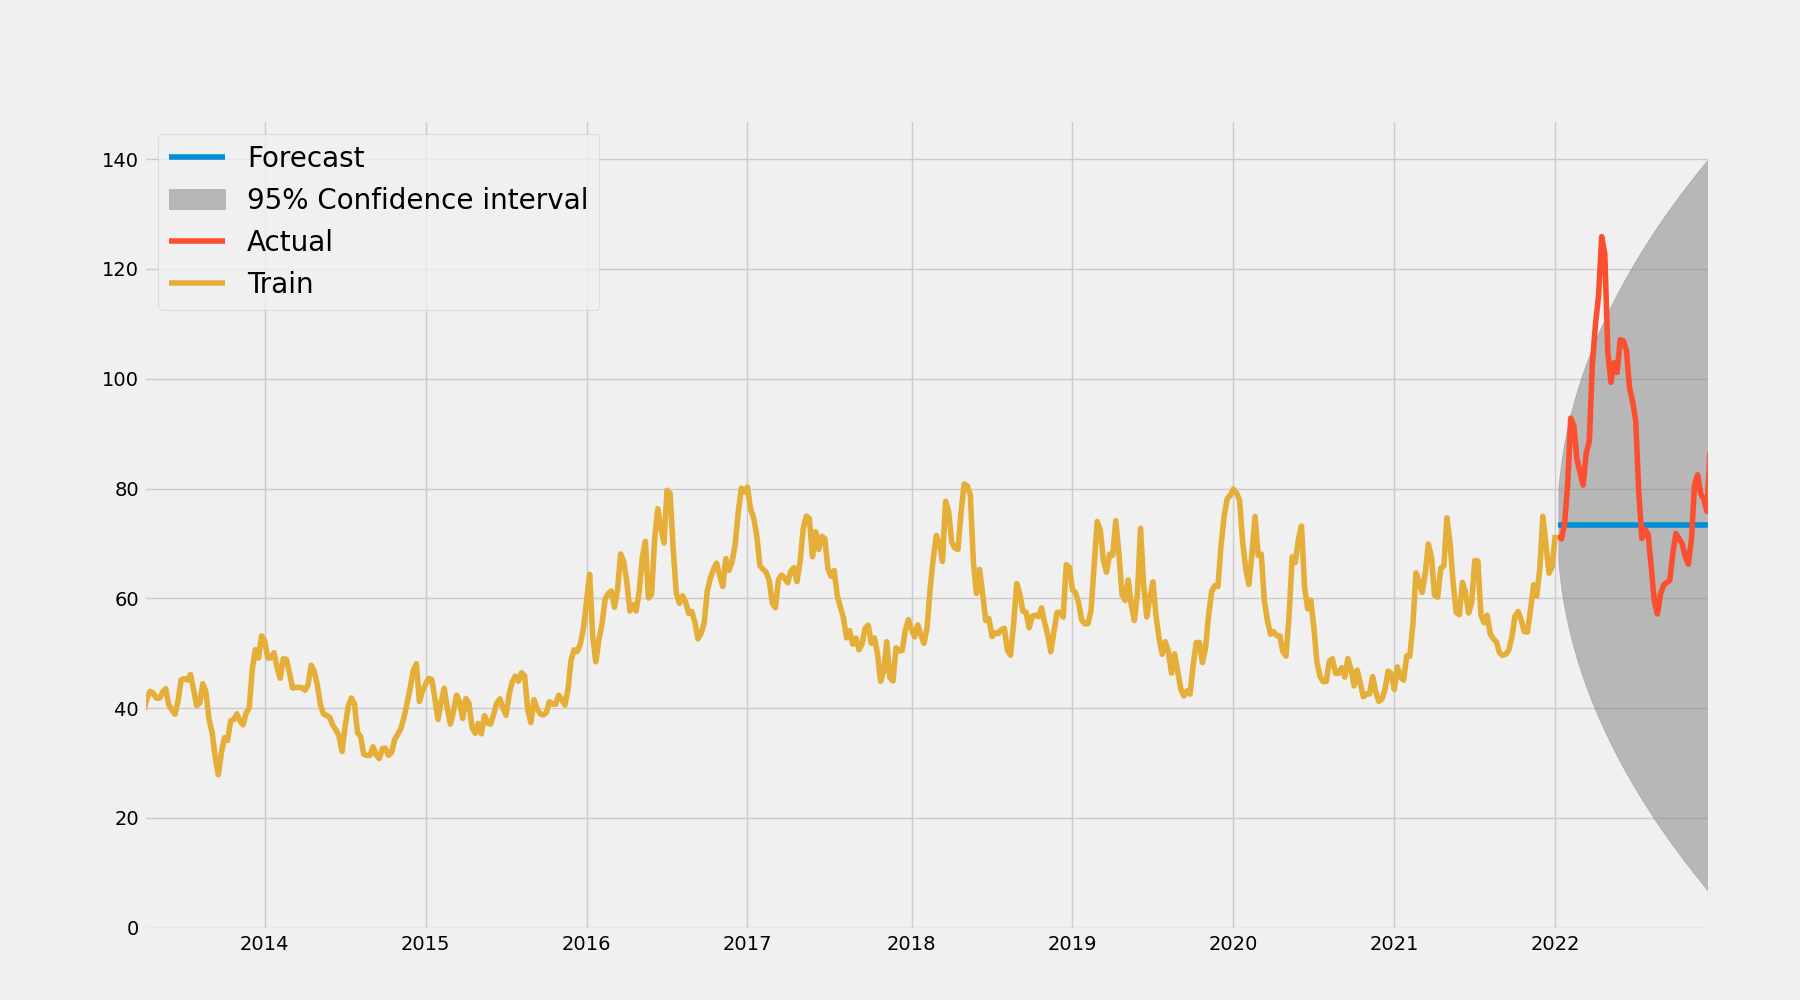
\includegraphics[width=0.9\textwidth]{data/Figures/ARIMA/ARIMA_0_1_1.png}
        \caption{ARIMA(0,1,1) model fitted to the data.}\label{fig:ARIMA_011}
    \end{center}
\end{figure}
As we can see, the model was not able to capture the trend, it seems that it was only able to take the average and draw it further out. In addition, the 95\% confidence interval is very wide, indicating that the model is less than accurate.

Since this was the ARIMA model with the lowest RMSE, there is no reason to believe that the other ARIMA models will be any more accurate. We will therefore not examine the other ARIMA models, but instead move on to the SARIMA models.

\subsection{SARIMA}\label{sec:sarima}
One of the more prominent features of the Salmon data is the clear seasonality that is exhibited on a yearly basis. We should therefore expect a seasonal model to better be able to capture this trend. As we did with the ARIMA models, we will perform a grid search on the different parameters using a nested for-loop, the problem with this is that the SARIMA model has 6 parameters instead of 3. The search will therefore grow exponentially. Consequently, we decided to solely use a $P$ of 0, $D$ of 1 and $Q$ of 0 as a larger $P$ and $Q$ seemed to have a negative effect on the RMSE. As the data has a seasonality of 52 weeks, this is the seasonal parameter we will use. The ten best results of the grid search are presented in the following table:
\begin{table}[H]
    \begin{center}
        \import{data/Figures/ARIMA/}{AutoSARIMAResults}
        \caption{Results of the grid search for the SARIMA model.}\label{tab:SARIMAResults}
    \end{center}
\end{table}
Similarly, to the ARIMA model, there is not a significant difference between the models, but the RMSE is clearly lower for the SARIMA than the ARIMA, this indicates the importance of capturing the seasonal trend in the dataset. The SARIMA(2,1,0)(0,1,0)[52] model has the lowest RMSE and should therefore be the most accurate SARIMA model. After fitting the model on the train data and comparing the predictions against the actual data we get the following plot:
\begin{figure}[H]
    \begin{center}
        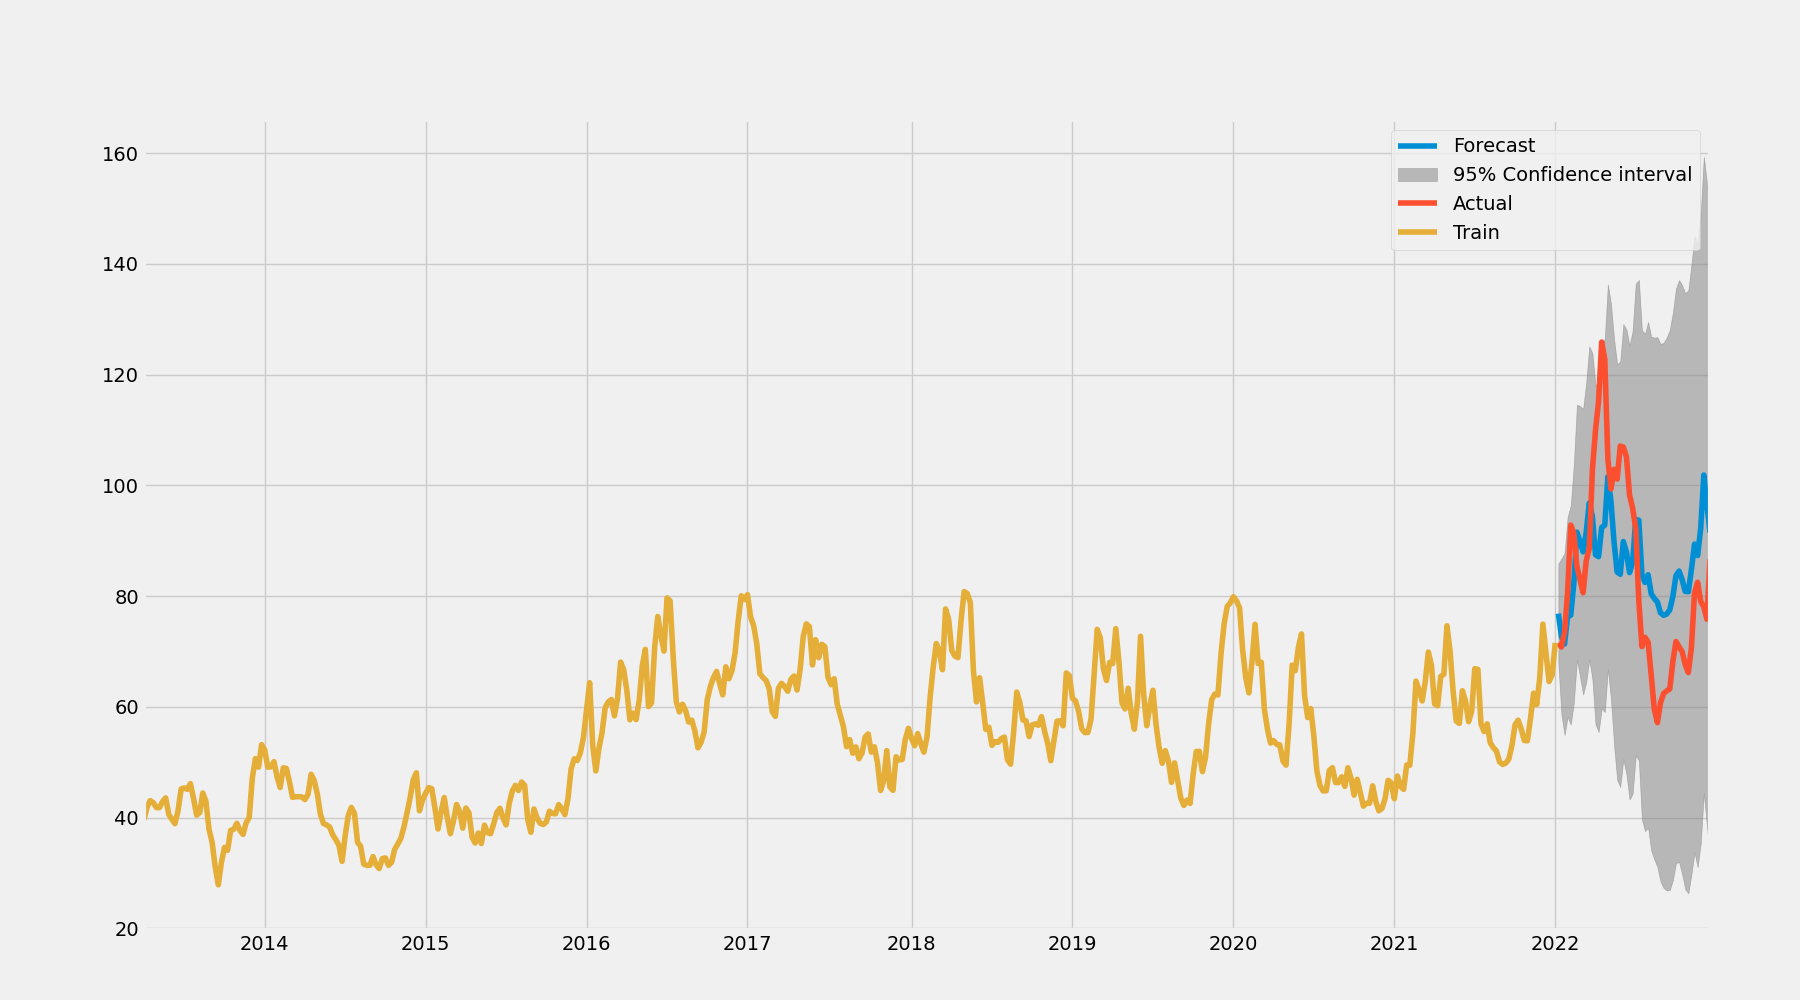
\includegraphics[width=0.9\textwidth]{data/Figures/ARIMA/SARIMA_2_1_0_0_1_0_52.png}
        \caption{SARIMA(2,1,0)(0,1,0,52) model fitted to the data.}\label{fig:SARIMA_21001052}
    \end{center}
\end{figure}
As we can see in figure~\ref{fig:SARIMA_21001052}, and as predicted from the RMSE, the SARIMA model is able predict the data much closer to the actual data than the ARIMA model. The 95\% confidence interval is still quite large, especially when we reach the end of 2022, but as we can see from the large spike in the spring of 2022, this interval is necessary to be accurate. We can also take a closer look at the twenty first predictions for the year 2022:
\begin{table}[H]
    \begin{center}
        \import{data/Figures/ARIMA/}{SARIMAForecastTable2}
        \caption{SARIMA(2,1,0)(0,1,0,52) model predictions for the year 2022.}\label{tab:SARIMA_forecast}
    \end{center}
\end{table}
Sorting the difference between actual and predicted values in ascending order we can see that the model does have some large errors, especially in the spring of 2022 with the largest difference being -33.5. We can also take a look at the actual model with the different parameters:

\begin{table}
    \begin{center}
        \begin{tabular}{lclc}
        \toprule
        \textbf{Dep. Variable:}          &          SalmonPrice           & \textbf{  No. Observations:  } &    457      \\
        \textbf{Model:}                  & SARIMA(2, 1, 0)x(0, 1, 0, 52) & \textbf{  Log Likelihood     } & -1190.4   \\
        \textbf{Date:}                   &        Fri, 21 Apr 2023        & \textbf{  AIC                } &  2386.72   \\
        \textbf{Time:}                   &            14:19:24            & \textbf{  BIC                } &  2398.73   \\
        \textbf{Sample:}                 &           04-07-2013           & \textbf{  HQIC               } &  2391.48   \\
        \textbf{}                        &          - 01-02-2022          & \textbf{                     } &             \\
        \textbf{Covariance Type:}        &              opg               & \textbf{                     } &             \\
        \bottomrule
        \end{tabular}
        \begin{tabular}{lcccccc}
                        & \textbf{coef} & \textbf{std err} & \textbf{z} & \textbf{P$> |$z$|$} & \textbf{[0.025} & \textbf{0.975]}  \\
        \midrule
        \textbf{ar.L1}  &       0.1953  &        0.044     &     4.486  &         0.000        &        0.110    &        0.281     \\
        \textbf{ar.L2}  &      -0.2932  &        0.043     &    -6.895  &         0.000        &       -0.376    &       -0.210     \\
        \textbf{sigma2} &      21.2106  &        1.328     &    15.966  &         0.000        &       18.607    &       23.814     \\
        \bottomrule
        \end{tabular}
        \begin{tabular}{lclc}
        \textbf{Ljung-Box (L1) (Q):}     & 0.14 & \textbf{  Jarque-Bera (JB):  } &  6.15  \\
        \textbf{Prob(Q):}                & 0.71 & \textbf{  Prob(JB):          } &  0.05  \\
        \textbf{Heteroskedasticity (H):} & 2.14 & \textbf{  Skew:              } & -0.14  \\
        \textbf{Prob(H) (two-sided):}    & 0.00 & \textbf{  Kurtosis:          } &  3.54  \\
        \bottomrule
        \end{tabular}
        \caption{SARIMA(2, 1, 0)x(0, 1, 0, 52) Results}\label{tab:SARIMA_summary}
    \end{center}
\end{table}
We can in table~\ref{tab:SARIMA_summary} see our two autoregressive terms, ar.L1 and ar.L2, and the error term sigma2. The important thing to note from the table is that both the autoregressive terms have a p-value of 0.000, which means that they are both statistically significant. Another important conclusion to draw from the SARIMA results is whether or not the residuals are independent, or white noise. Examining the Ljung-Box test, we see that it produces a result with a p-value of 0.71, this is far greater than the critical value of 0.005. This means that we cannot reject the null hypothesis that the residuals are independent, and there could therefore be more information in the residuals that the model was not able to capture. 

While the AIC and BIC values both can be important to when comparing models, the change in differencing and seasonality makes it difficult to compare the models purely based on this criterion. This is part of the reason why we chose to use the RMSE as our main criterion for comparing the models.
\subsection{SARIMAX}\label{sec:sarimax}
The final way to improve upon our ARIMA model is to include exogenous variables. We will also here utilize a grid search on the different parameters in order to optimize the model. To reduce the number of iterations we will assume that the optimal parameters from the SARIMA model are still the optimal parameters for the SARIMAX model. Further, we have the choice between having all exogenous variables in the model, only a few, or just a single variable. We will start by including all exogenous variables in the model, and then gradually reduce the number of exogenous variables. As there is only one possible model when including all models, we will not use a grid search, but instead just fit the model, we then get the following results:
\begin{table}[H]
    \begin{center}
        \import{data/Figures/ARIMA/}{SARIMAX_all_RMSE_df}
        \caption{Result from SARIMAX model with all exogenous variables.}\label{tab:SARIMAX_all}
    \end{center}
\end{table}
As we can see from table~\ref{tab:SARIMAX_all} the RMSE did increase from table~\ref{tab:SARIMAResults}, this probably means that the exogenous variables do not increase the accuracy of the model. This might be because there are conflicting trends in the exogenous variables that cancel each other out. A better way to increase accuracy might therefore be to drop some of the exogenous variables and instead include the ones that reduces the RMSE the most. Iterating over all possible combinations of two exogenous variables we get the following results:
\begin{table}[H]
    \begin{center}
        \import{data/Figures/ARIMA/}{SARIMAX_multi_RMSE_df}
        \caption{Result from SARIMAX model with two exogenous variables.}\label{tab:SARIMAX_multi}
    \end{center}
\end{table}
Examining the RMSE we can now see that reducing the number of variables had a positive effect on the accuracy of the model. We archived the best results when including HalibutPrice and TWI as exogenous variables. This might indicate that the CodPrice has a negative effect on the model. In addition, this SARIMAX model is more accurate than the SARIMA model, which indicates that the inclusion of exogenous variables can improve the accuracy. 

Still, we can reduce the number of exogenous variables to just one, in order possibly improve the accuracy even further. Utilizing a grid search we get the following results:
\begin{table}[H]
    \begin{center}
        \import{data/Figures/ARIMA/}{SARIMAX_uni_RMSE_df_assume}
        \caption{Result from SARIMAX model with one exogenous variable.}\label{tab:SARIMAX_uni}
    \end{center}
\end{table}
As we can see, the RMSE did improve. More interestingly, it seems that the only exogenous variable that improves the accuracy of the model is the TWI, as both HalibutPrice, CodPrice and CPI has a negative effect on the model. To examine the results further we can take a look at the summary of the model:
\begin{table}[H]
    \begin{center}
        \begin{tabular}{lclc}
        \toprule
        \textbf{Dep. Variable:}          &          SalmonPrice           & \textbf{  No. Observations: } &    457      \\
        \textbf{Model:}                  & SARIMAX(2, 1, 0)x(0, 1, 0, 52) & \textbf{  Log Likelihood    } & -1185.0  \\
        \textbf{Date:}                   &        Sun, 23 Apr 2023        & \textbf{  AIC               } &  2378.09   \\
        \textbf{Time:}                   &            17:10:51            & \textbf{  BIC               } &  2394.09   \\
        \textbf{Sample:}                 &           04-07-2013           & \textbf{  HQIC              } &  2384.42   \\
        \textbf{}                        &          - 01-02-2022          & \textbf{                     } &             \\
        \textbf{Covariance Type:}        &              opg               & \textbf{                     } &             \\
        \bottomrule
        \end{tabular}
        \begin{tabular}{lcccccc}
                        & \textbf{coef} & \textbf{std err} & \textbf{z} & \textbf{P$> |$z$|$} & \textbf{[0.025} & \textbf{0.975]}  \\
        \midrule
        \textbf{TWI}    &      -0.5192  &        0.146     &    -3.561  &         0.000        &       -0.805    &       -0.233     \\
        \textbf{ar.L1}  &       0.1774  &        0.043     &     4.087  &         0.000        &        0.092    &        0.263     \\
        \textbf{ar.L2}  &      -0.3044  &        0.044     &    -6.850  &         0.000        &       -0.391    &       -0.217     \\
        \textbf{sigma2} &      20.6612  &        1.320     &    15.650  &         0.000        &       18.074    &       23.249     \\
        \bottomrule
        \end{tabular}
        \begin{tabular}{lclc}
        \textbf{Ljung-Box (L1) (Q):}     & 0.05 & \textbf{  Jarque-Bera (JB):  } &  5.29  \\
        \textbf{Prob(Q):}                & 0.82 & \textbf{  Prob(JB):          } &  0.07  \\
        \textbf{Heteroskedasticity (H):} & 2.04 & \textbf{  Skew:              } & -0.17  \\
        \textbf{Prob(H) (two-sided):}    & 0.00 & \textbf{  Kurtosis:          } &  3.45  \\
        \bottomrule
        \end{tabular}
        \caption{SARIMAX(2, 1, 0)x(0, 1, 0, 52) Results}
    \end{center}
\end{table}
Compared to table~\ref{tab:SARIMA_summary}, we can see that both the AIC and BIC have been reduced. This does indicate that the model is more accurate. However, the p-value of the Ljung-Box test is still above the critical value of 0.05 which indicates that the residuals are not white noise and that there might be some trends left in the residuals that the model has not captured.

Finally, we can plot the results from the best SARIMA and SARIMAX model against the actual data:
\begin{figure}[H]
    \centering
    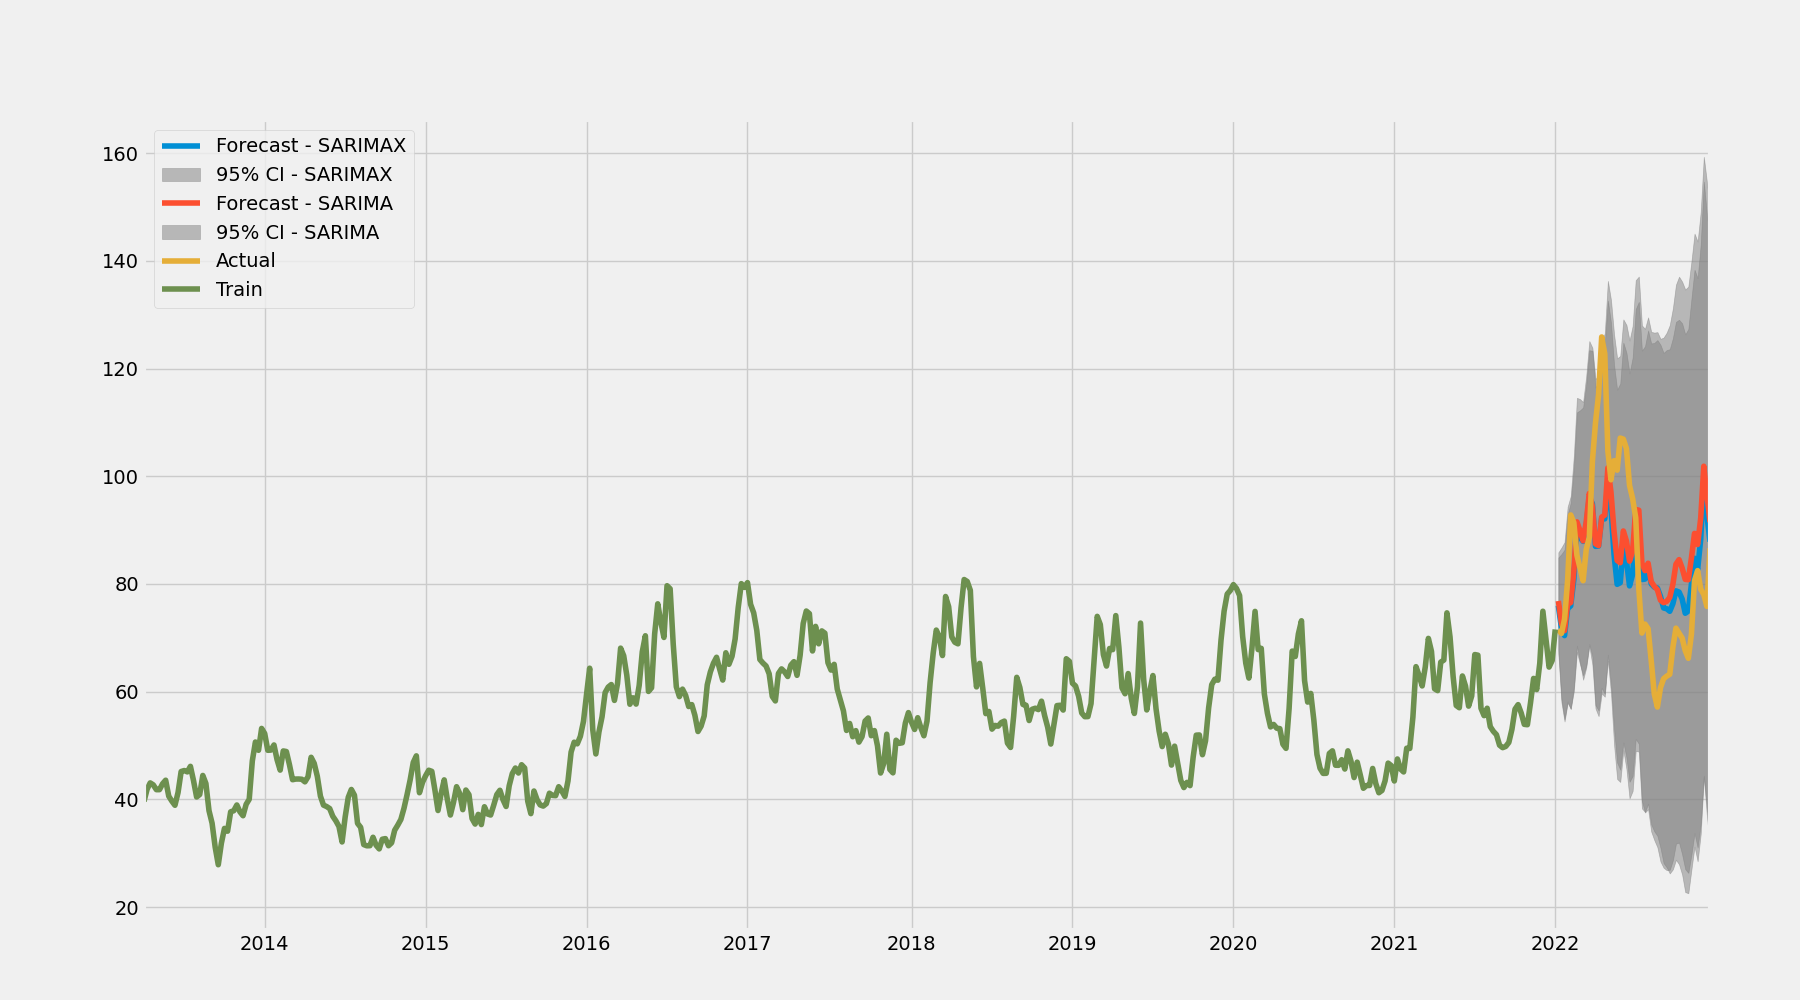
\includegraphics[width=0.8\textwidth]{data/Figures/ARIMA/SARIMA-SARIMAX.png}
    \caption[SARIMAX(2,1,0)(0,1,0,52)(TWI) compared with SARIMA.]{SARIMAX model with TWI as exogenous variable compared with SARIMA.}\label{fig:SARIMA-SARIMAX}
\end{figure}
\begin{figure}[H]
    \centering
    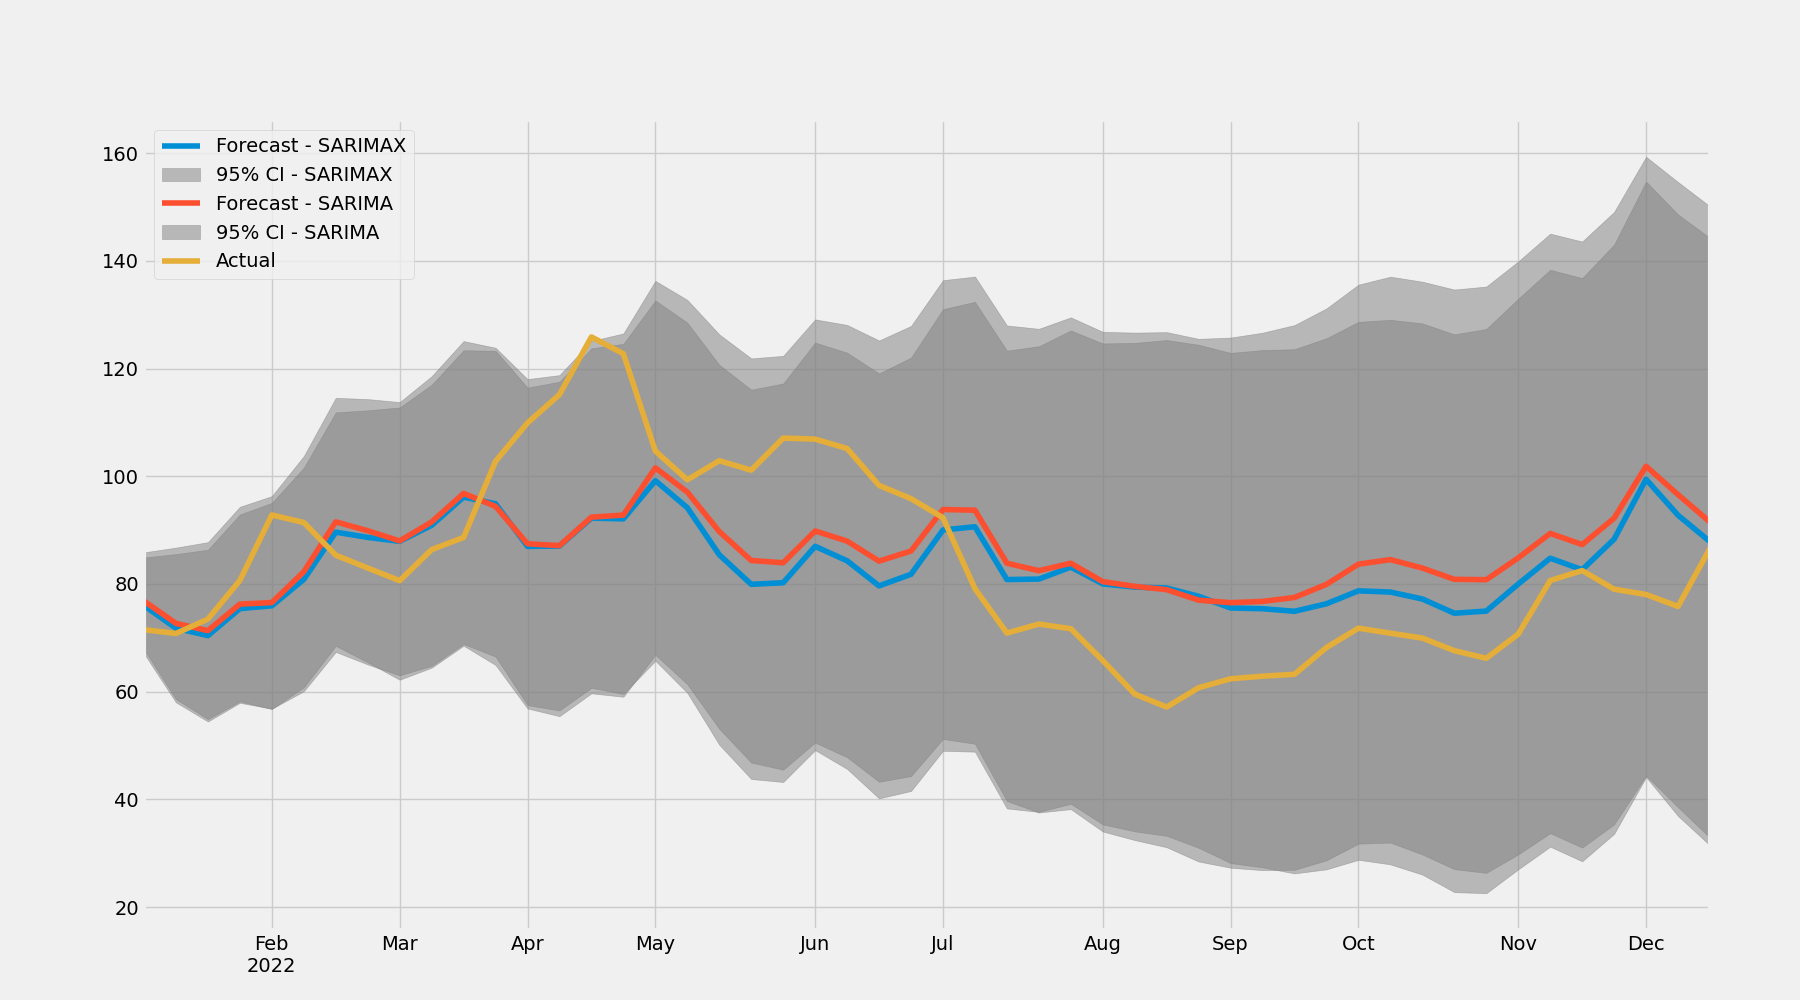
\includegraphics[width=0.8\textwidth]{data/Figures/ARIMA/SARIMA-SARIMAX_no_train.png}
    \caption{Predictions from figure~\ref{fig:SARIMA-SARIMAX}.}\label{fig:SARIMA-SARIMAX_no_train}
\end{figure}
Comparing these predictions we find no discernible difference between the two models. This is not surprising with a difference in RMSE of only 0.3. The reason why the SARIMAX model is somewhat more accurate may be that it throughout predicts a lower price than the SARIMA model.

\subsection{LSTM}\label{sec:lstm}
In order to get a meaningful result from the different models in the grid search, the RMSE was calculated for each model, and returned to the following dataframe:
\begin{table}[H]
    \centering
    \begin{adjustbox}{width=\columnwidth,center}
    \import{"data/Figures/Neural networks/"}{RMSE_Tensorflow_head}
    \end{adjustbox}
    \caption{RMSE for each model in the grid search.}\label{tab:RMSE_Tensorflow_head}
\end{table}
These first runs are not particularly accurate, at least compared to the best SARIMAX models. There are also no clear difference between the different parameters. A more efficient way to find the best models is sorting after the RMSE. This is done in the following table:
\begin{table}[H]
    \centering
    \begin{adjustbox}{width=\columnwidth,center}
    \import{"data/Figures/Neural networks/"}{RMSE_Tensorflow_top}
    \end{adjustbox}
    \caption{RMSE for each model in the grid search sorted after RMSE.}\label{tab:RMSE_Tensorflow}
\end{table}
By examining table~\ref{tab:RMSE_Tensorflow} we can clearly see that the best performing LSTM model is run number 186 with a batch size of 26, 100 epochs, 52 timesteps and with the nadam optimizer. Still, the RMSE is somewhat worse than the best SARIMAX model. This may indicate that the neural network was not able to capture all the trends in the dataset. 

An interesting observation is that while the SARIMA and SARIMAX were quite similar measured by RMSE, every single of the best LSTM models are multivariate. The LSTM may therefore be better suited for multivariate time series than univariate, and may need a larger amount of data to be able to capture the trends. 

\begin{figure}[H]
    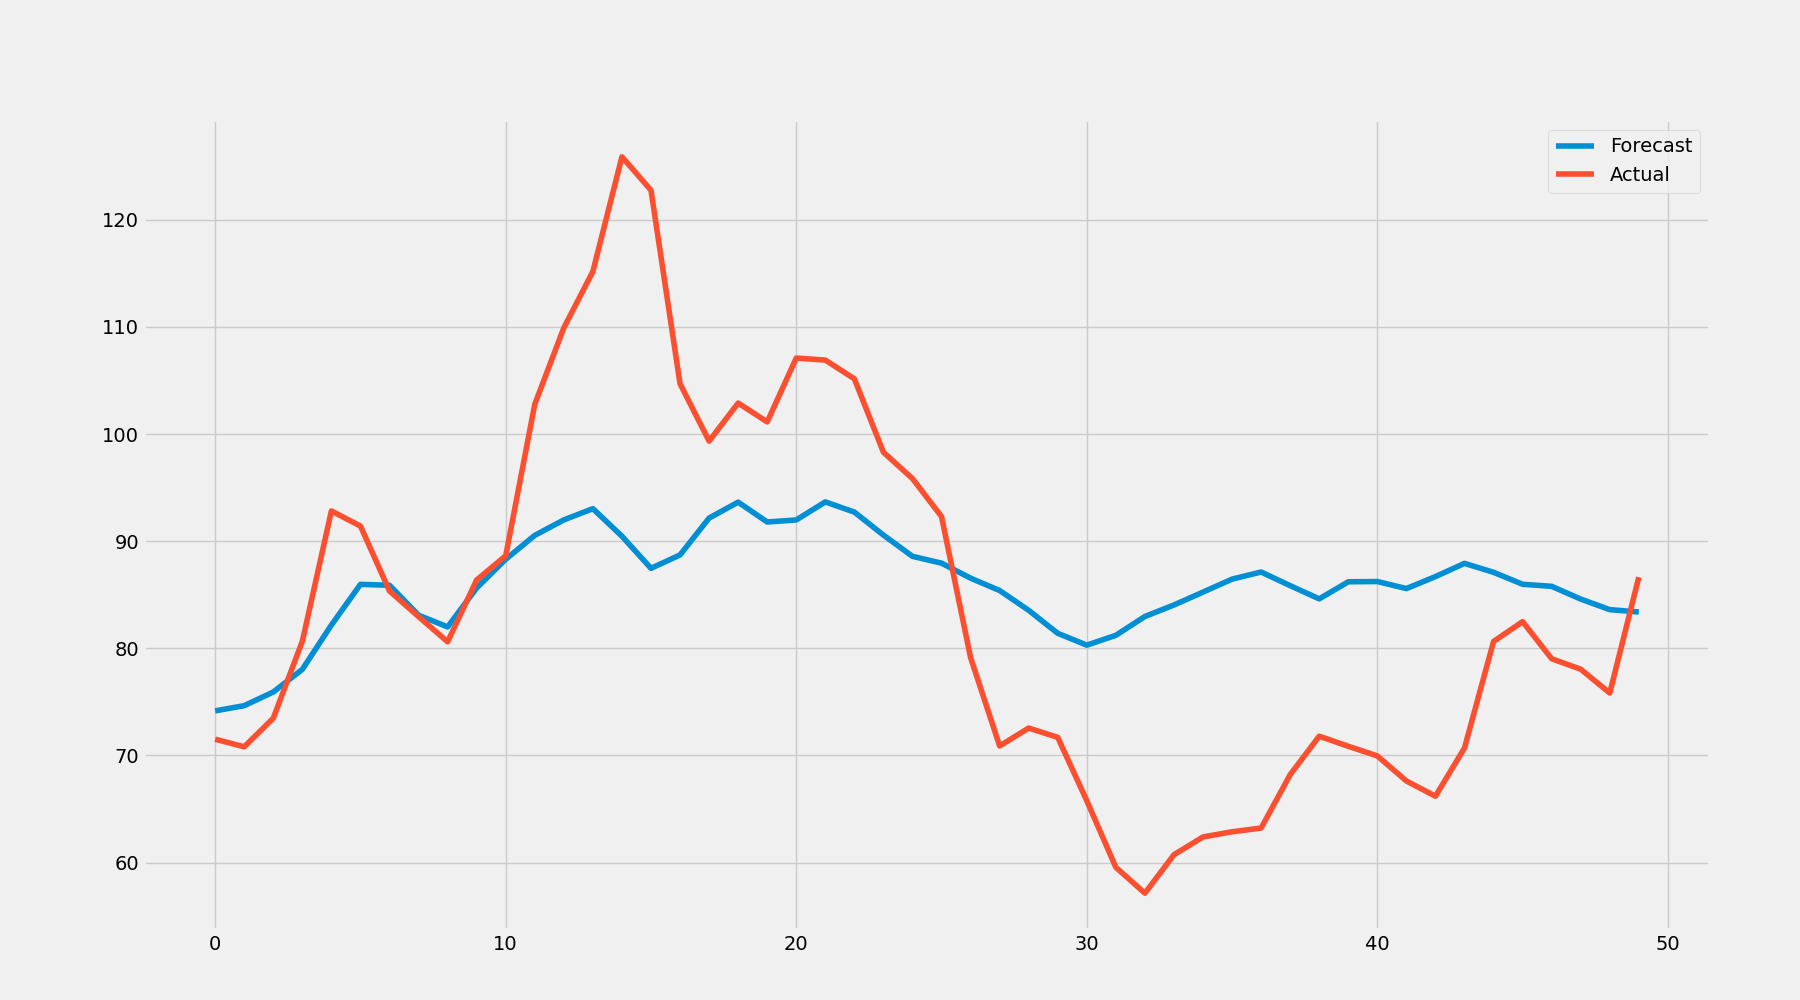
\includegraphics[width=.48\textwidth]{../data/Figures/Neural networks/ForLoop_Tensor/plotModel_186.png}\hfill
    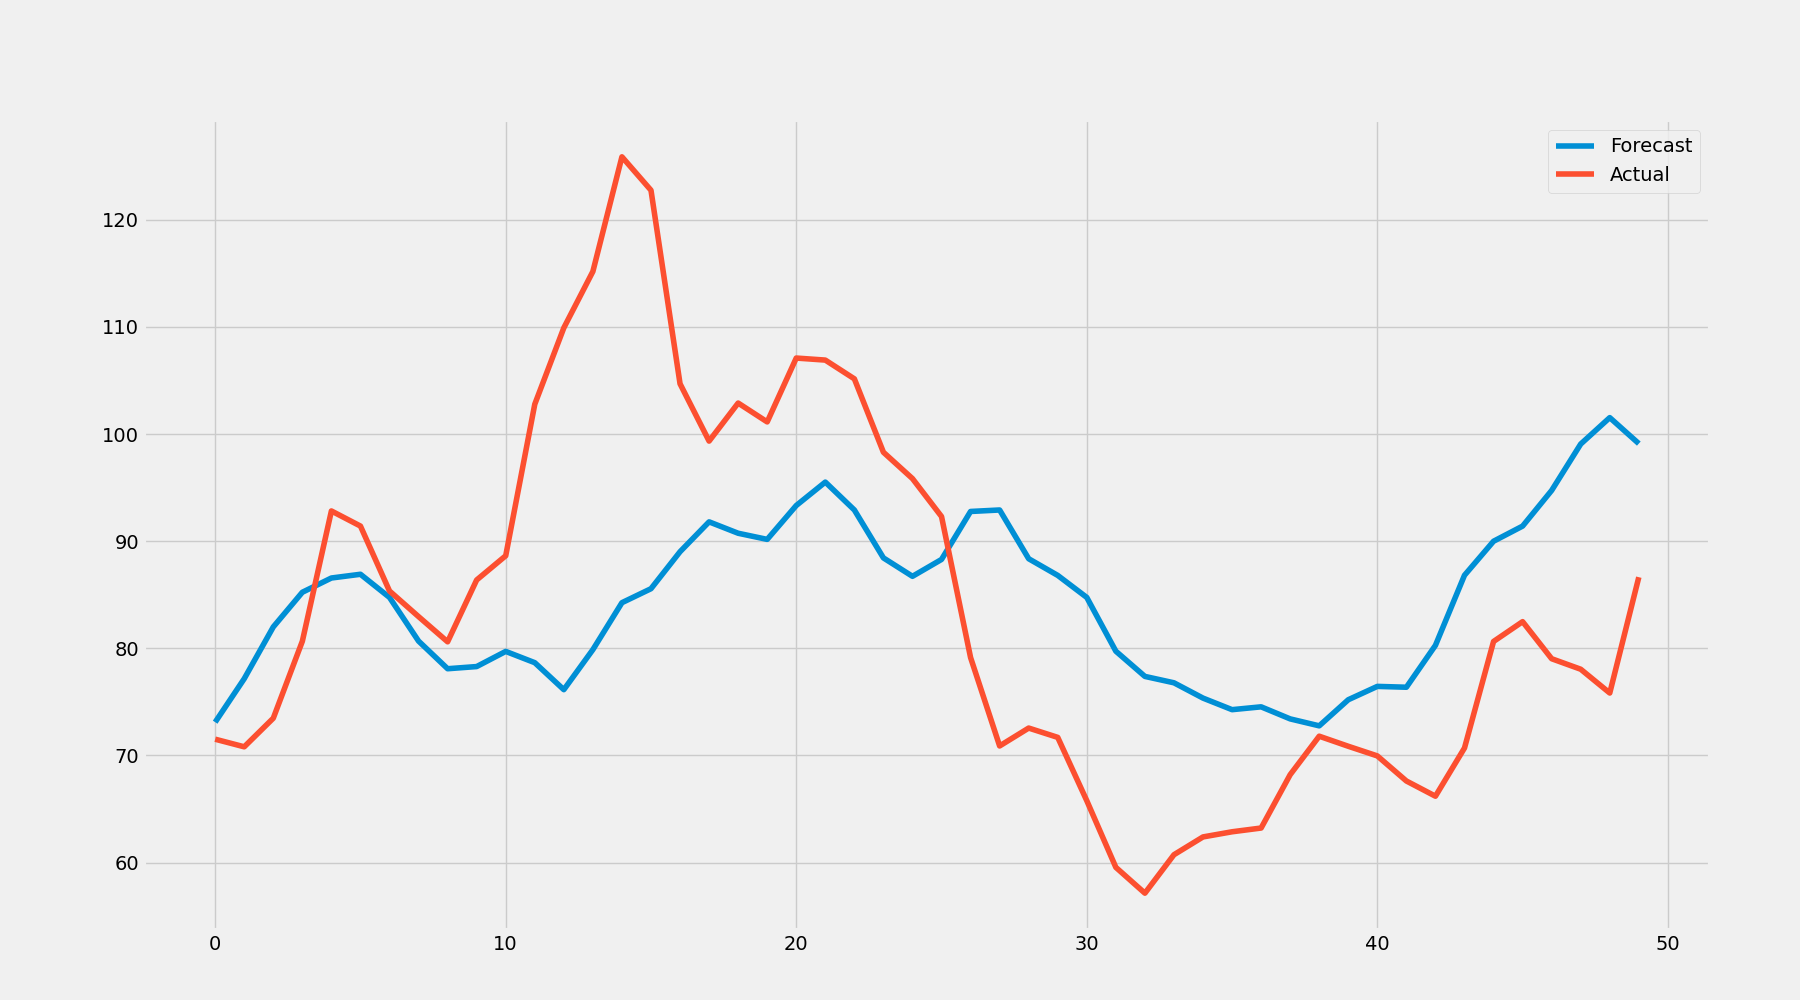
\includegraphics[width=.48\textwidth]{../data/Figures/Neural networks/ForLoop_Tensor/plotModel_72.png}\hfill
    \\[\smallskipamount]
    \includegraphics[width=.48\textwidth]{../data/Figures/Neural networks/ForLoop_Tensor/plotmodel_286.png}\hfill
    \includegraphics[width=.48\textwidth]{../data/Figures/Neural networks/ForLoop_Tensor/plotmodel_46.png}
    \captionsetup{justification=centering}
    \caption[The eight best models measured by RMSE, 1--4]{The eight best models measured by RMSE, 1--4, actual data in red, predicted data in blue}\label{fig:best_models14}
\end{figure}

\begin{figure}[H]
    \includegraphics[width=.48\textwidth]{../data/Figures/Neural networks/ForLoop_Tensor/plotmodel_202.png}\hfill
    \includegraphics[width=.48\textwidth]{../data/Figures/Neural networks/ForLoop_Tensor/plotmodel_124.png}\hfill
    \\[\smallskipamount]
    \includegraphics[width=.48\textwidth]{../data/Figures/Neural networks/ForLoop_Tensor/plotmodel_130.png}\hfill
    \includegraphics[width=.48\textwidth]{../data/Figures/Neural networks/ForLoop_Tensor/plotmodel_52.png}
    \captionsetup{justification=centering}
    \caption[The eight best models measured by RMSE, 5--8]{The eight best models measured by RMSE, 5--8, actual data in red, predicted data in blue}\label{fig:best_models58}
\end{figure}

\vspace{\baselineskip}
By plotting the models from table~\ref{tab:RMSE_Tensorflow} we can see that the four best models are able to quite accurately predict the next year, while the next four models does not seem to capture any other trend than a rolling mean. The RMSE from these models may therefore be somewhat misleading as they are not able to capture any complex trends. 

In order to determine the effect of the different hyperparameters we can group by these and calculate the mean RMSE for each group. This is done in the following tables:
\begin{table}[H]
    \centering
    \import{"data/Figures/Neural networks/"}{RMSE_Batch_size}
    \caption{Mean RMSE for each batch size.}\label{tab:RMSE_batch_size}
\end{table}

\begin{minipage}{.5\textwidth\relax}
    \begin{table}[H]
        \centering
        \import{"data/Figures/Neural networks/"}{RMSE_Time_steps}
        \caption{Mean RMSE for each timestep.}\label{tab:RMSE_Tensorflow_groupby_timesteps}
    \end{table}
    \end{minipage}%
\begin{minipage}{.5\textwidth\relax}
\begin{table}[H]
    \centering
    \import{"data/Figures/Neural networks/"}{RMSE_Epochs}
    \caption{Mean RMSE for each epoch.}\label{tab:RMSE_epochs}
\end{table}
\end{minipage}%

\begin{minipage}{.5\textwidth\relax}
\begin{table}[H]
    \centering
    \import{"data/Figures/Neural networks/"}{RMSE_Optimizer}
    \caption{Mean RMSE for each optimizer.}\label{tab:RMSE_optimizer}
\end{table}
\end{minipage}%
\begin{minipage}{.5\textwidth\relax}
\begin{table}[H]
    \centering
    \import{"data/Figures/Neural networks/"}{RMSE_UniMulti}
    \caption{Mean RMSE for each univariate or multivariate model.}\label{tab:RMSE_uni_multi}
\end{table}
\end{minipage}%

From the different tables we can discern that there are not any large difference in RMSE between the different hyperparameters. With the exception of univariate to multivariate where the multivariate models do have a clear lower RMSE. An interesting conclusion to draw is that the batch size seem to have a small effect on the RMSE, and it may therefore be more efficient with a large batch size, as this should decrease the computational time needed. Another is that the number of time steps does not have a large effect on the RMSE, even though we hypothesised that it may see more seasonality when introducing more time steps. This may still be attributed to the models ability to capture the rolling trend of the data in such a way that the RMSE becomes somewhat misleading.

The number of epochs in table~\ref{tab:RMSE_epochs} does not seem to vary from 10 to 40, but seems to have some effect when increasing to 100 epochs. This may either be due to the need for more epochs to draw out the information from the data, especially with such a simple model, or it may be because of overfitting of the data. Taking a look at the loss plot from the same models we examined in figure~\ref{fig:best_models14} and~\ref{fig:best_models58} we see that for the models with an actual variation in the prediction there is a logarithmic decrease, converging towards 0 loss. Comparatively, the models where the predictions are more similar to a rolling mean, the loss exhibits a large amount of variation. This may indicate that the model is not able to learn anything from the data, and is therefore not able to improve the prediction. 

Interestingly, several of the models that perform well in terms of RMSE, have an optimal epoch of 40. This might indicate that the loss will increase with more epochs. 
\begin{figure}[H]
    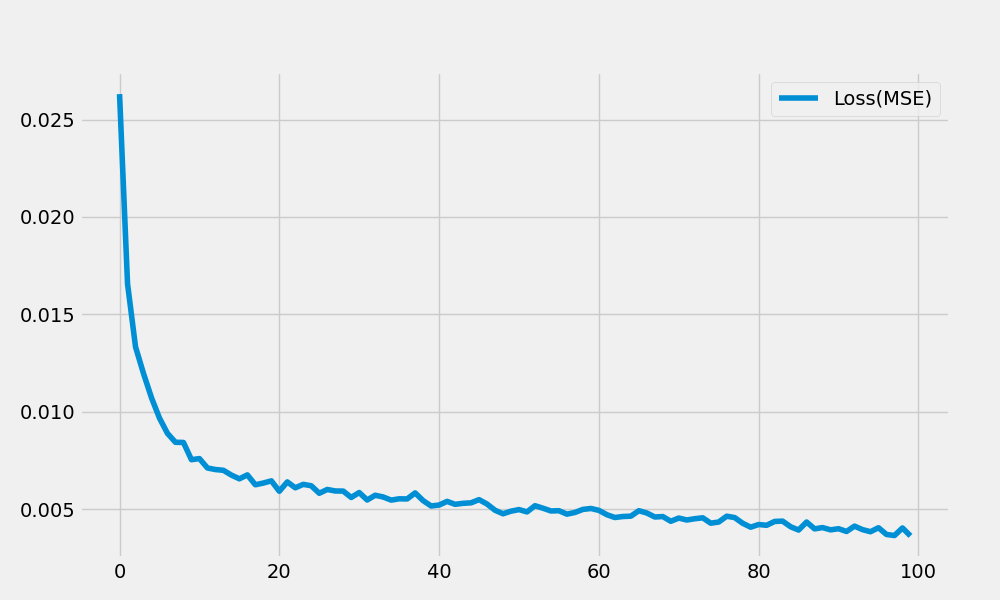
\includegraphics[width=.48\textwidth]{../data/Figures/Neural networks/ForLoop_Tensor/plotLoss_186.png}\hfill
    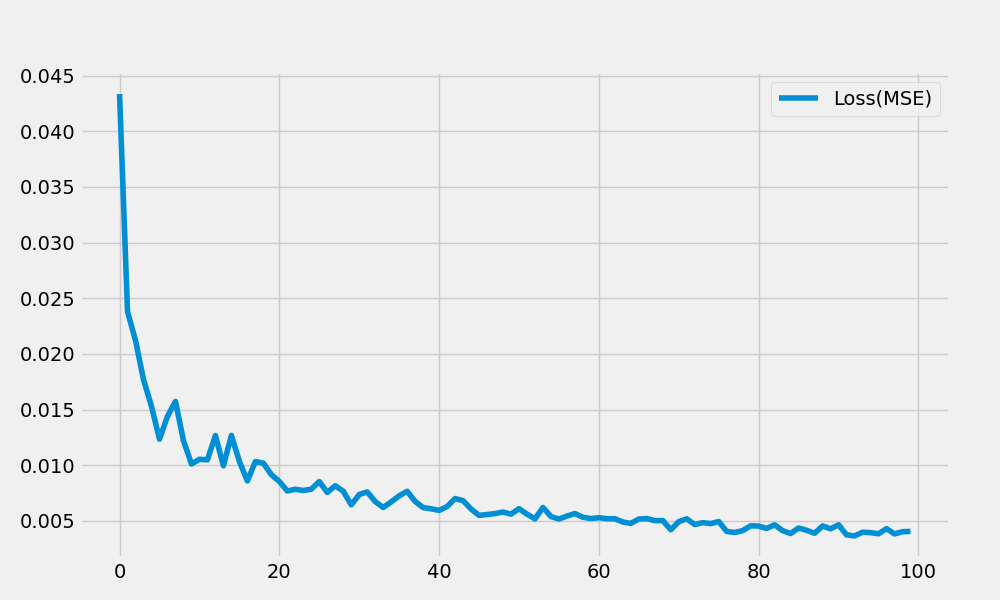
\includegraphics[width=.48\textwidth]{../data/Figures/Neural networks/ForLoop_Tensor/plotLoss_72.png}\hfill
    \\[\smallskipamount]
    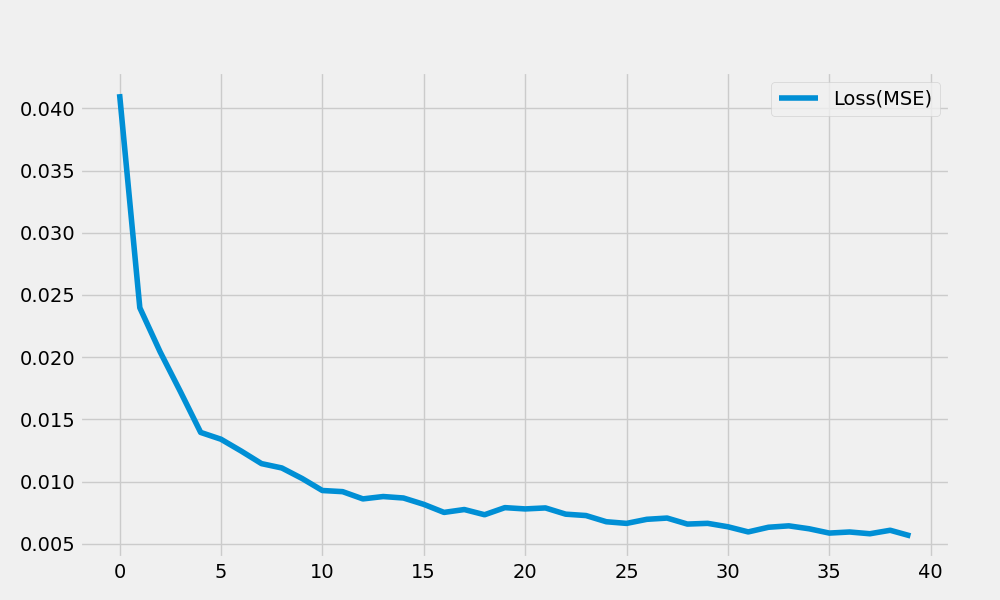
\includegraphics[width=.48\textwidth]{../data/Figures/Neural networks/ForLoop_Tensor/plotLoss_286.png}\hfill
    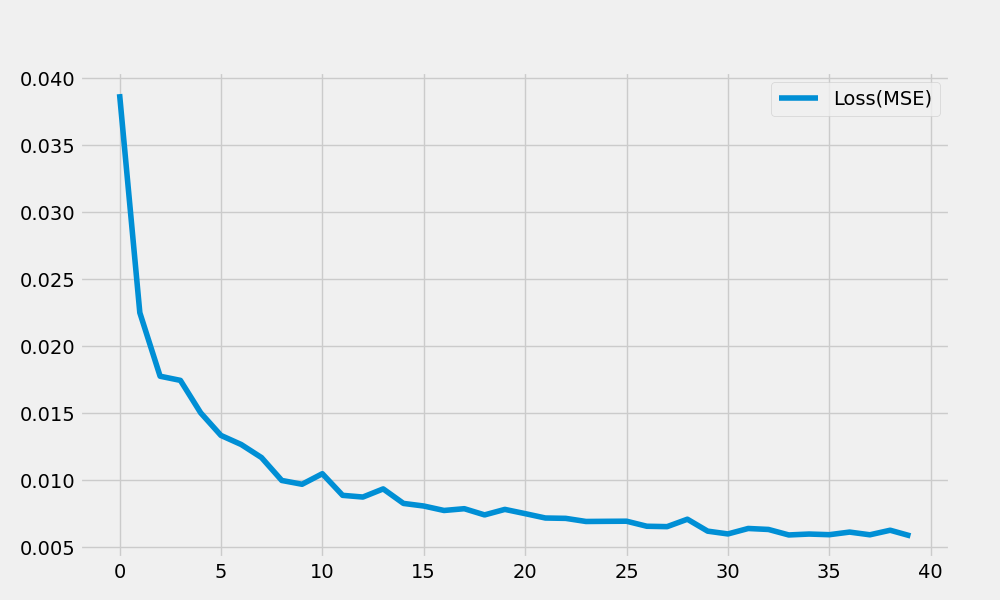
\includegraphics[width=.48\textwidth]{../data/Figures/Neural networks/ForLoop_Tensor/plotLoss_46.png}\caption{Loss plot for the eight best models measured by RMSE, 1--4}\label{fig:loss_14}
\end{figure}
\begin{figure}
    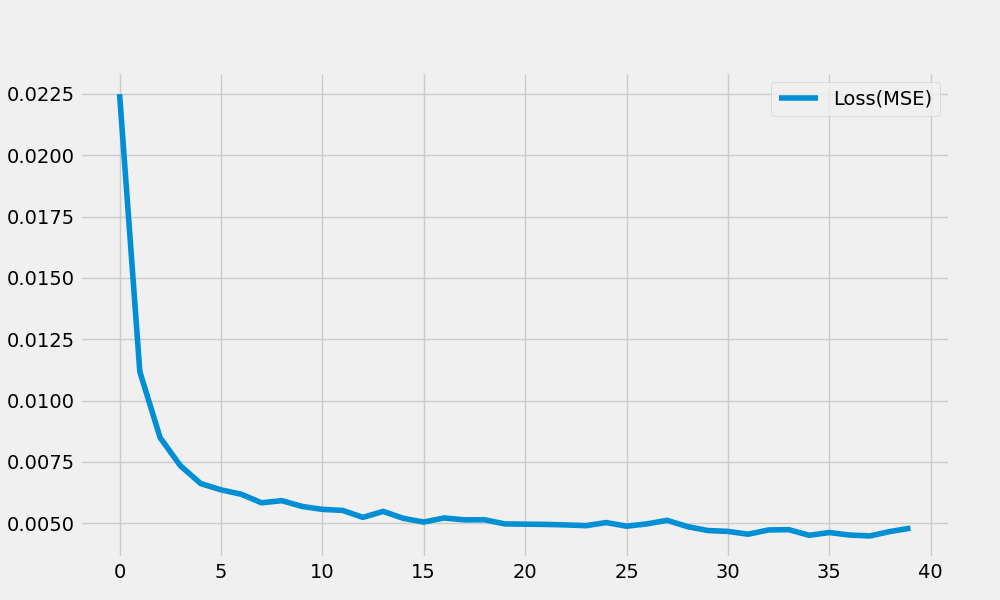
\includegraphics[width=.48\textwidth]{../data/Figures/Neural networks/ForLoop_Tensor/plotLoss_202.png}\hfill
    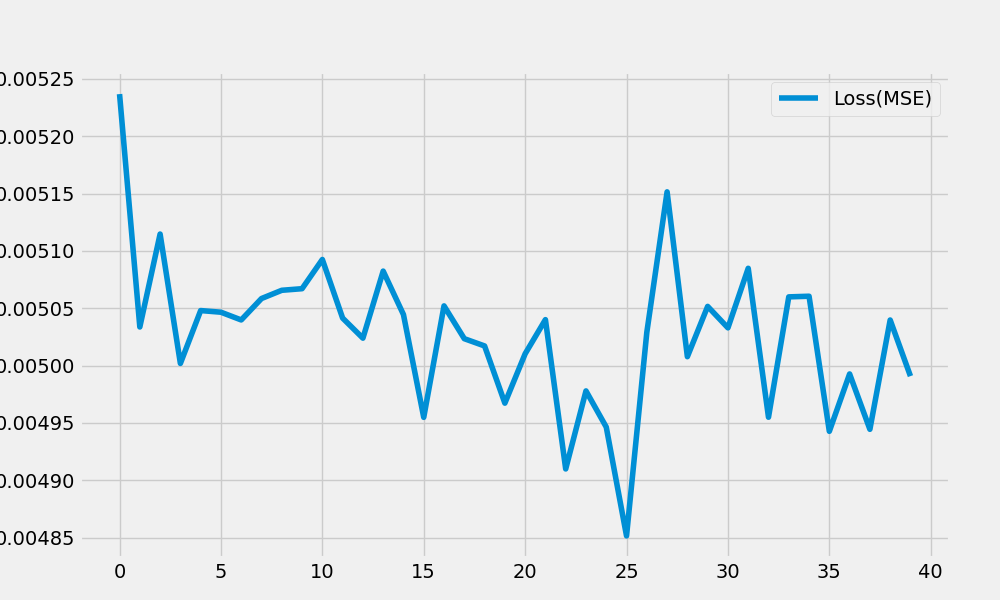
\includegraphics[width=.48\textwidth]{../data/Figures/Neural networks/ForLoop_Tensor/plotLoss_124.png}\hfill
    \\[\smallskipamount]
    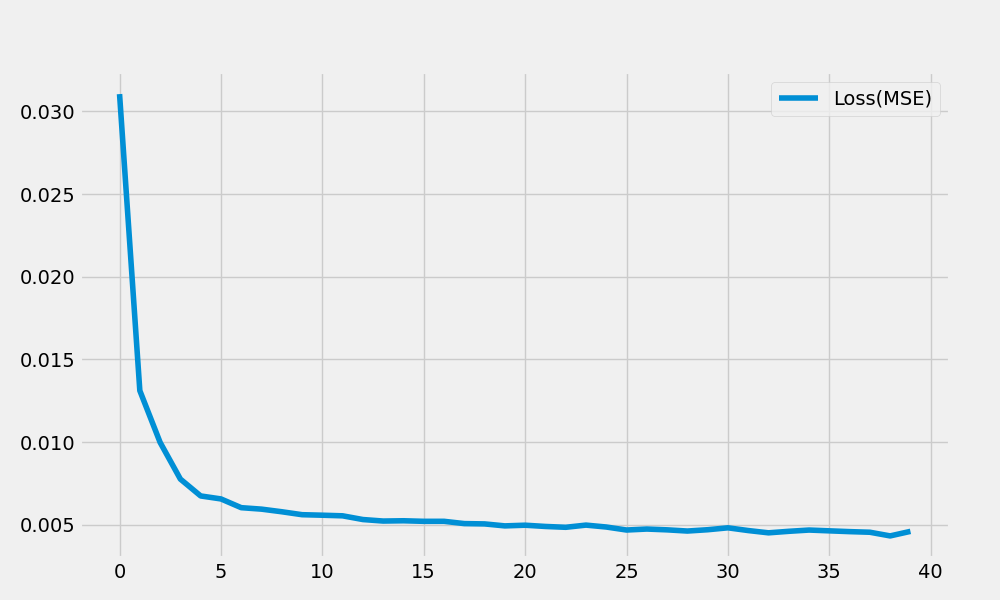
\includegraphics[width=.48\textwidth]{../data/Figures/Neural networks/ForLoop_Tensor/plotLoss_130.png}\hfill
    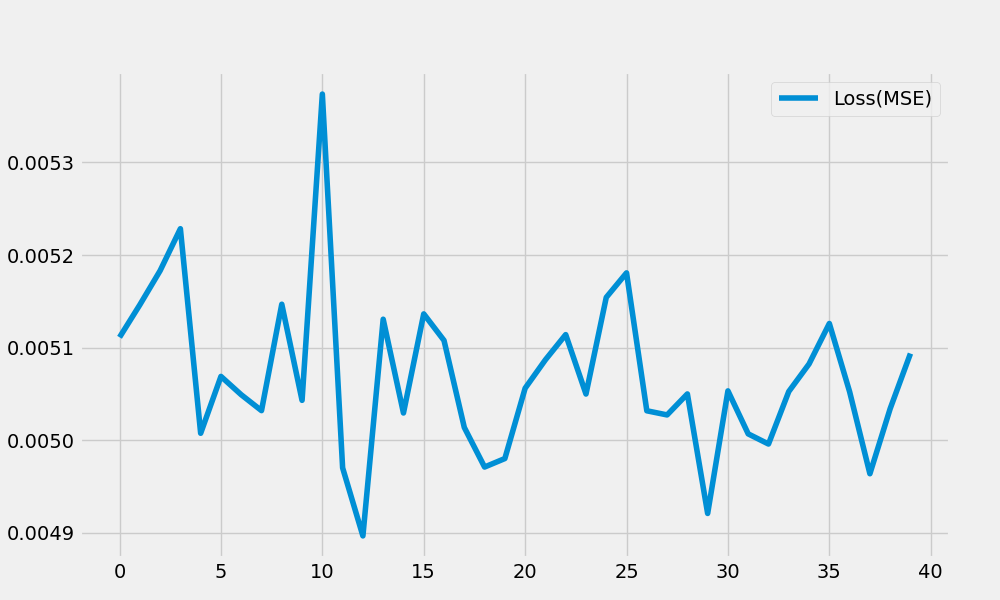
\includegraphics[width=.48\textwidth]{../data/Figures/Neural networks/ForLoop_Tensor/plotLoss_52.png}\caption{Loss plot for the eight best models measured by RMSE, 5--8}\label{fig:loss_58}
\end{figure}

\subsection{Comparison and Discussion}\label{sec:comparison}

The biggest difference in RMSE is from ARIMA to SARIMA, indicating the importance of seasonality. Adding exogenous variable to the SARIMA, making it a SARIMAX model, improves the RMSE very slightly, but the SARIMAX model still seems to be suboptimal. Comparing the RMSE from the SARIMAX model and the LSTM model we see that the best prediction from the LSTM is still slightly worse than the SARIMAX model. This being said there is a little drop off in the RMSE from the best prediction from the LSTM to the second best, meaning that cherry picking the best prediction from the LSTM gives a wrong impression of how well the LSTM actually performs. At the same time its also worth noting that without the lack of the necessary computing power, as well as the other limitations listed below, the LSTM model has the potential to be the best model.

One limitation in our data is the massive swings of the salmon price in 2022. Compared to earlier years we see that the trends are still the same in 2022, but the extent of the price-spikes are much larger. This means that actually producing a model that predicts the price in 2022 relatively well would mean that the model is in fact not very good. Good models would have to produce lower highs and higher lows than what was actually the case in 2022. This is the case for our test set aswell, and is very clearly illustrated in figure \ref{fig:SARIMA-SARIMAX_no_train} where the actual price is peaking outside of the 95\% confidence interval. In order to succeed in predicting such a steep climb in price with certainty the model would have to capture a much larger portion of the factors that go into determining the price.

Given that the NASDAQ gathers it data though sampling form a large range of sales venues each week and by doing so aggregating a good average with little bias over time. This might cause the low look back LSTM models to be biased in some of its predictions because it looks at this small sample isolated. This can be one the reasons the model is not able to catch the trends as well in the low look back ranges. 

Even though our best model, the SARIMAX, seems to be somewhat able to catch the trends, we cant say that there is not more information in the residuals. The results from the Ljung-Box test means that we have to reject the null hypothesis. However, rejecting the null hypothesis only tells us that we cant claim that there is not white noise. It does not mean that we can claim that there is white noise. This uncertainty means that we cant be sure how much of the price fluctuations are explained by the model and how much is left in the residuals. 

When suggesting further research we note that when
examining the Ljung-Box test on the SARIMAX model. It shows that the residuals might not be white noise, and that there might be some trends left to capture. We therefore suggest that future research focuses on improving the models and perhaps lengthen the dataset in order to get better odds of picking up these more illusive trends. One possibility for improving the models is simply to use more computing power as this would allow for more complex models. Another possibility is to use different variables in the multivariate analysis in LSTM as we saw the multivariate was by far the best version of LSTM. This might also apply to the SARIMAX model. It is possible to try different models entirely, but we suggest focusing on multivariate.